\chapter{Detector Installation and Commissioning Organization}
\label{ch:tc-jpo}

As discussed in Chapter~\ref{vl:tc-global}, the \dword{ipd} has
responsibility for coordinating the planning and execution of 
\dword{lbnf-dune} integration and installation activities both 
in the underground detector caverns at \dword{surf} and in the 
nearby surface facilities.  The \dword{dune} consortia maintain 
responsibility for their subsystems over the course of these 
activities and provide the expert personnel and specialized 
equipment necessary to integrate, install, and commission their 
detector components.  Likewise, \dword{lbnf} has responsibility 
for activities associated with the integration and installation 
of supporting infrastructure items, which are coordinated under 
the direction of the \dword{ipd}.       

The \dword{jpo} will evolve over time to incorporate the team in South 
Dakota responsible for the overall coordination of on-site integration 
and installation activities.  In the meantime, the installation team 
within the \dword{jpo} works directly with the \dword{dune} consortia 
and \dword{lbnf} project team members to plan out these activities.  
\dword{jpo} installation team members are concurrently embedded 
within the \dword{dune} \dword{tc} organization during this period to 
facilitate required interactions with the \dword{dune} consortia. 

The \dword{jpo} team responsible for installation planning is additionally 
responsible for the specification and procurement of common infrastructure 
items associated with the integration and installation of the detectors, 
which are not included within the scope of the \dword{dune} consortia.  
Some of these items are detector pieces such as racks, cable trays, cryostat 
flanges, and the mechanical structures for supporting the detectors within 
the cryostats.  Others are general items required for detector integration 
and installation such as clean rooms, cranes, scaffolding, and personnel 
lifts.  Within its support role, \dword{dune} \dword{tc} works closely with 
the \dword{jpo} team to characterize these items and contributes engineering 
resources for required design efforts.

The on-site \dword{jpo} team that will take responsibility for coordinating
integration and installation activities at \dword{surf} will include rigging 
teams responsible for moving materials in and out of the shaft, through the 
underground drifts, and within the detector caverns.  It will also include 
prersonnel responsible for overseeing safety and logistics planning.  These 
team members are anticpated to sit within the \dword{sdsd}, an organization 
formed to provide \dword{fnal} support services in South Dakota.    

\section{Far Site Safety}
\label{sec:far_site_safety}

The foundation of a credible integration and installation plan is 
an \dword{esh} program that ensures the safety of particpating team 
members, the equipment supporting the program, and the environment 
at the \dword{surf} site.  The \dword{ipd} has direct responsibility 
for implementing the \dword{lbnf-dune} \dword{esh} program within 
the planned integration and installation activities in South Dakota.  
The \dword{lbnf-dune} \dword{esh} Manager heads the on-site safety 
organization and reports directly to the \dword{ipd} to support them
in carrying out this responsibility.

An on-site \dword{esh} Coordinator sitting under the \dword{lbnf-dune} 
\dword{esh} Manager oversees the day to day execution of the integration 
and installation work and remains in direct communication with one of 
three safey officers assigned to each individual work shift.  The safety 
officer assigned to a particular shift is responsible for leading the 
safety discussions that take place during the daily toolbox meeting and 
for ensuring that all of the integration/installation workers on that 
shift, including those from the consortia, are properly trained.  The 
reporting chain for safety incidents goes directly through the on-site 
safety team to the \dword{lbnf-dune} \dword{esh} Manager to minimize 
any potential conflicts of interest.  All \dword{jpo} installation team 
members as well as \dword{dune} consortia personnel and \dword{lbnf} project 
team members have the right to stop work for any safety issues.

Documentation, including accident reports, near misses, weekly reports, 
equipment inspection, and training records is an important component of 
the \dword{lbnf-dune} \dword{esh} program.  Operation of all equipment 
used for integration and installation activities such as cranes, power 
tools, and personnel lifts is restricted to team members who have been
properly trained and certified for using that equipment.  The safety 
coordinator for each shift is responsible for ensuring that all team 
personnel are properly trained and that safety documentation and work 
procedures are up-to-date and stored within the \dword{edms}.  

The work planning and \dword{ha} program utilizes detailed work
plan documents, \dword{ha}  reports, equipment documentation,
safety data sheets, \dword{ppe} and job task training to mimimize work place
hazards and maximize efficiency.  This documentation is developed
through the \dword{ashriver} trial assembly process, which maps out the 
step by step procedures and brings together the documenation needed 
for approving the work plan.  Documentation is modified to account for  
differences required for performing work underground and the updated 
procedures are passed through \dwords{orr} from which   
\dwords{orc} for work to proceed can be 
obtained.

\section{JPO Management}
\label{vl:tc-facility_mgmt}

The \dword{ipd} is responsible for coordinating all integration and
installation activities at \dword{surf} including those that fall 
under the direct responsibility of \dword{lbnf} and the \dword{dune} 
consortia.  The coordinators of the different activities and crucial 
technical support staff sit within the \dword{jpo}.  The organization
of this on-site team is shown in shown in Figure~\ref{fig:ash_river}.  

\begin{dunefigure}[Far Site Organization Chart]{fig:ash_river}
  {Far Site Organization Chart}
  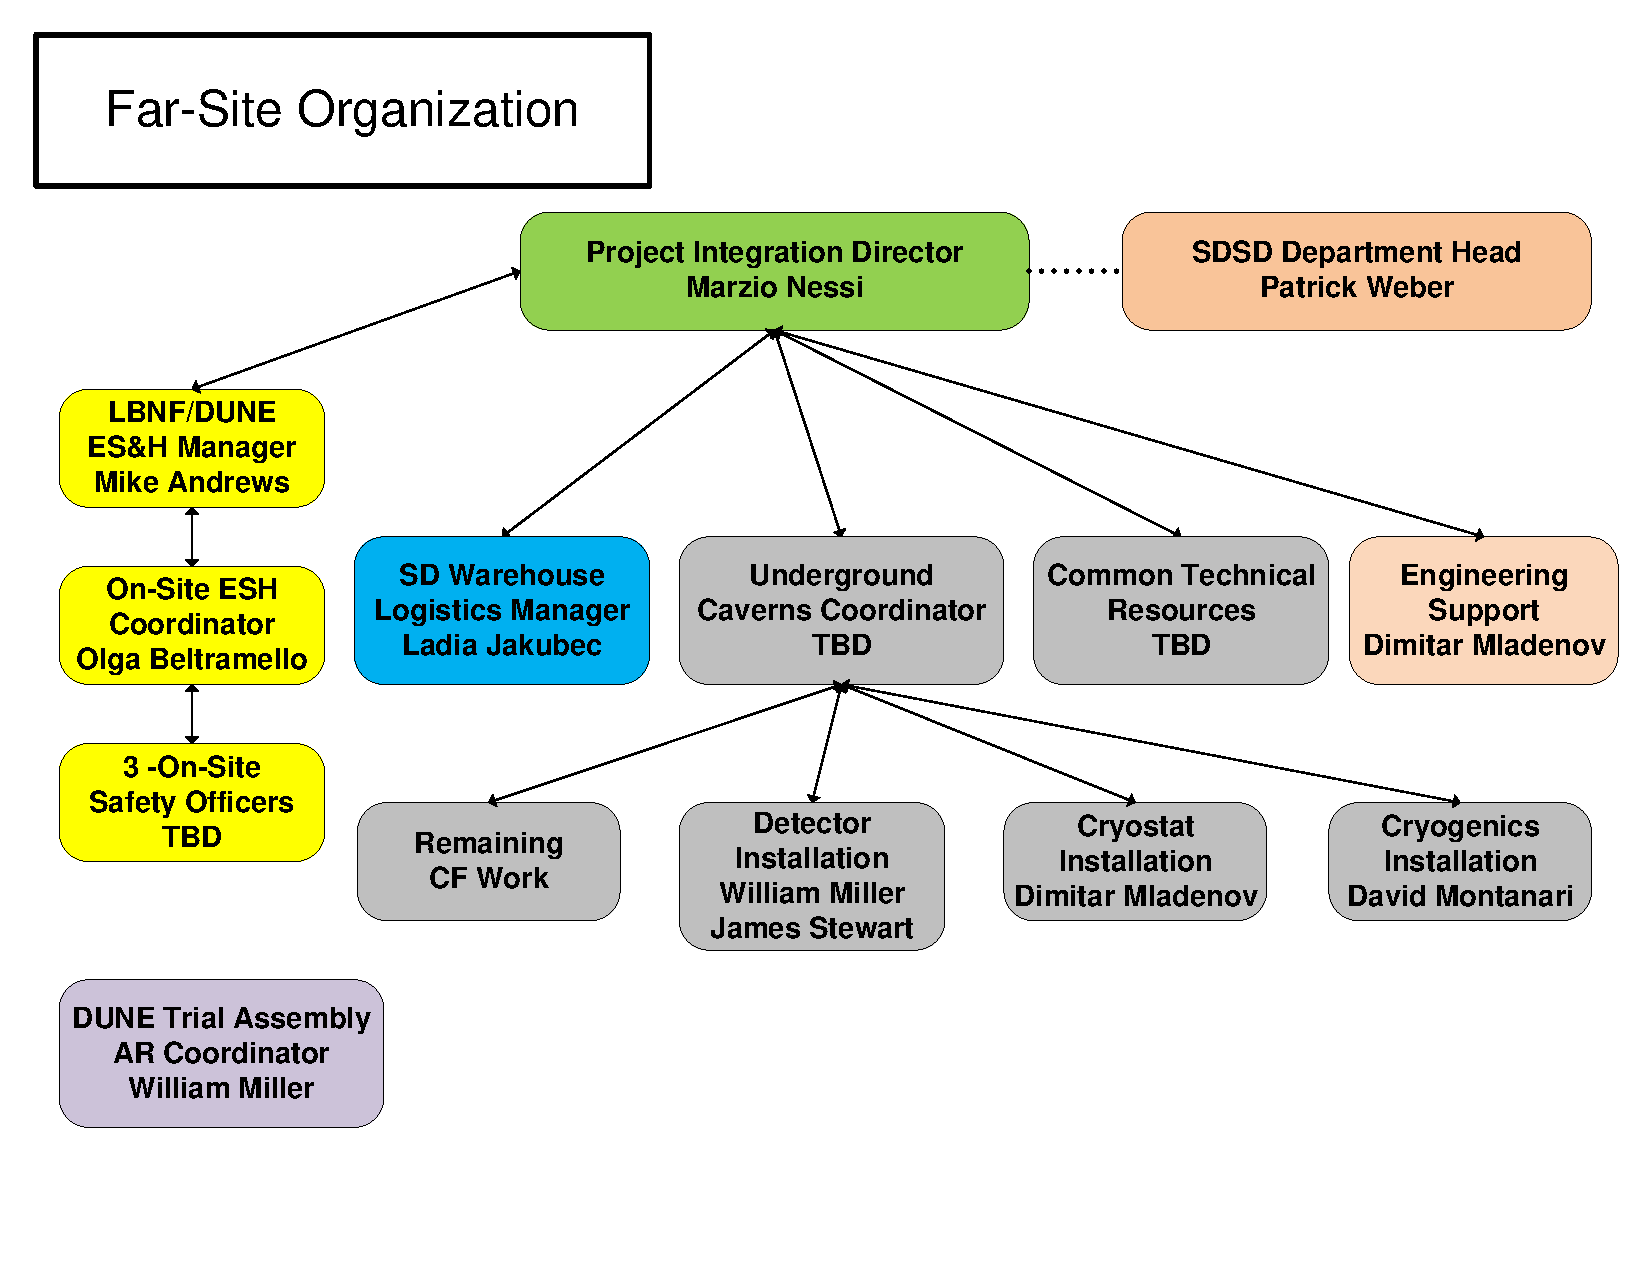
\includegraphics[width=0.95\textwidth]{Org-Far-Site-4-12-19.pdf}
\end{dunefigure}
 
As discussed in Section~\ref{sec:far_site_safety} an on-site safety 
organization incorporating an \dword{esh} Coordinator and three 
safety officers working under the direction of the \dword{lbnf-dune} 
\dword{esh} manager oversees all on-site activites and has a direct 
reporting line to the \dword{ipd}.  Due to the lack of surface space 
at \dword{surf}, a separate warehousing facility in the vicinity of 
\dword{surf} is required to receive and store materials in advance 
of their delivery to the undergound area.  Warehouse operations are 
coordinated by the \dword{lbnf-dune} logistics manager who is tasked 
with determining the exact sequence in which materials are delivered
into the underground areas.         

The underground caverns coordinator is responsible for managing all 
of the activities in the two undergound detector caverns as well as 
the \dword{cuc}.  Work within the detector caverns follows a time 
ordered sequence that includes installation of the cryostats (warm
and cold), cryogenic systems, and the detectors themselves.  Work 
in the \dword{cuc} includes installation of major cryogenic system 
pieces and the detector \dword{daq} electronics.  The underground 
caverns coordinator relies on separate installation teams focusing 
on cryostats, cryogenic systems, and the detectors.  The cryostat 
and cryogenics system installation teams are contracted resources 
provided by \dword{lbnf}.  For this reason, coordinators of these 
activities are embedded within both the \dword{lbnf} project team 
and the \dword{jpo}.  The detector installation teams incoporate a 
substantial number of scientific and technical personnel from the 
\dword{dune} consortia.  Coordinators of the detector installation 
effort sit directly within the \dword{jpo} during the period when 
these activities are being executed.  Any required improvements or 
upgrades to the detector caverns occuring after their beneficial 
occupancy are also managed by the underground caverns coordinator  
under the direction of the \dword{ipd}.

The \dword{ipd} manages common technical and engineering resources 
to support the integration and installation activities.  Technical
resources include the support crews needed for handling materials 
at the warehouse facility, rigging materials on and off the hoist 
at the top and bottom of the shaft, transporting materials to the
underground caverns from the bottom of the shaft, and rigging the 
detector and infrastructure pieces within the underground caverns 
during the installation process.  Additional, common technical 
resources used across the installation efforts are welders, 
survey teams, and cabling crews.  Access to on-call electricians, 
plumbers, and network technicians is also required to support 
the installation effort and deal with operational issues as they 
arise.  Required technical resources described here are provided 
through the \dword{sdsd}, which will host full-time staff members 
and contracted support staff to provide the necessary functions.     

Engineering resources for integration and installation activities 
sit directly within the \dword{jpo}.  The engineering team, which 
includes both mechanical and electrical engineers, is required to 
resolve last minute issues associated with component handling and 
detector grounding that arise over the course of the installation 
process.  Other required engineering functions include procurement
support, configuration managament, and particpation in the safety 
review process.

\subsection{South Dakota Warehouse Facility}

The \dword{sdwf} is a leased 5000m$^2$ facility hosted by the
\dword{sdsd}.  Approximately six months before benficial occupancy 
of the underground detector caverns is received, the \dword{sdwf} 
is required to be in place for receiving cryostat and detector 
components.  Laydown space near the Ross headframe is extremely 
limited.  For this reason, the transportation of materials from 
the \dword{sdwf} to the top of the Ross shaft requires careful 
coordination. The \dword{lbnf-dune} logistics manager works with 
the \dword{cmgc}, through the end of excavation activities, and 
the other members of the \dword{jpo} team to coordinate transport 
of materials into the underground areas.  Since no materials or 
equipment can be shipped directly to the Ross or Yates headframes, 
the \dword{sdwf} is used for both short and long-term storage, as 
well as for any re-packaging of items required prior to transport 
into the underground areas. 

The organization responsible for managing activites at the 
\dword{sdwf} is shown in Figure~\ref{fig:sdwf}.  The facility 
coordinator works closely with the \dword{lbnf-dune} logistics 
manager and underground caverns coordinator to transport the 
correct items to \dword{surf} for transport into the underground
areas on an as needed basis.  Proper scheduling of shipments is 
critical due to the fact that the surface area around the Ross 
headframe can only accomodate one or two trucks at a time.   

\begin{dunefigure}[South Dakota Warehouse Facility team]{fig:sdwf}
  {South Dakota Warehouse Facility team}
  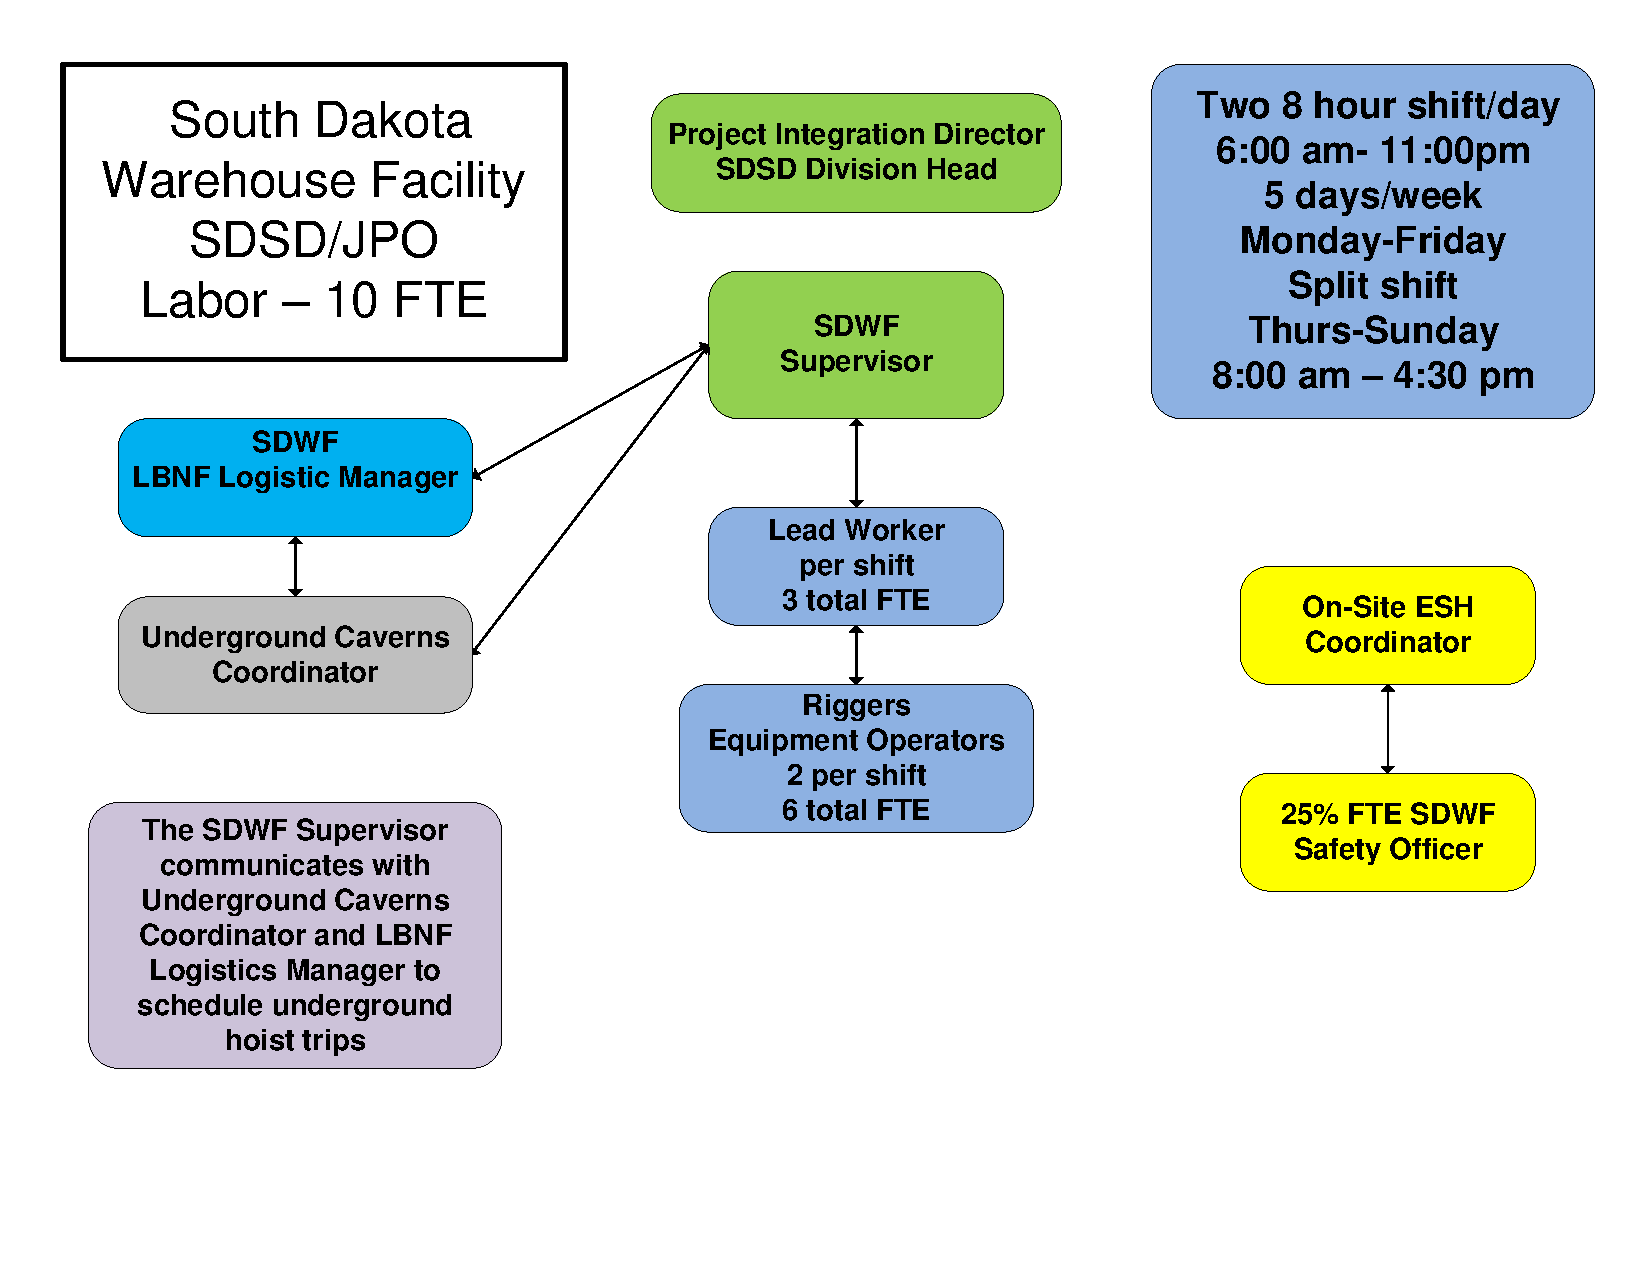
\includegraphics[width=0.95\textwidth]{Org_SDWF-4-5-19v2.pdf}
\end{dunefigure}

The \dword{sdwf} is operated seven days per week, with two shifts 
per day Monday thru Friday and a split day shift on the weekends 
to optimally overlap with shaft operations at \dword{surf}, which 
are twenty-four hours per day, seven days per week.  Activities at
the \dword{sdwf} are managed by the facility coordinator who has  
three lead workers to cover all shifts and a small crew of trained 
riggers and equipment operators to provide the required materials 
handling functions.  

A small number of \dword{dune} consortia members also work out of 
the \dword{sdwf} to check received components for potential damage 
incurred during shipment and track, using the inventory management 
system, all materials coming in and out of the facility.  In some 
cases re-packaging of materials is required for lowering them down
the shaft into the underground areas.  The \dword{dune} consortia
also take responisbility for these efforts, which are additionally
supported by the \dword{sdwf} operations crew.   

The on-site safety officers are responisible for overseeing the 
activities at the \dword{sdwf} under the direction of the on-site 
\dword{esh} coordinator.  The safety officer covering a specific 
shift has responsibility for ensuring that all of the \dword{sdwf}
personnel are properly trained and holding daily or weekly toolbox 
meetings as needed.

\subsection{Underground Caverns}

As discussed in Sec.~\ref{vl:tc-facility_mgmt}, the installation 
process in the underground detector caverns and \dword{cuc} can 
be broken into a time-sequenced set of activities, coordinated 
through the \dword{jpo}.  In the detector caverns, installation 
of the warm and cold cryostat strucutres is followed by (with 
some overlap) installation of the cryogenic infrastrucutre and 
detectors.  In the \dword{cuc} installation of the \dword{daq}  
infrastrucutre and detector readout components proceeds in 
parallel with that of the cryogenic infrastructure.  A high-level 
schedule showing the inter-dependencies between these activities 
is shown in Figure~\ref{fig:underground_schedule}.

\begin{dunefigure}[Underground summary schedule]{fig:underground_schedule}
  {Summary schedule or the different phases of work underground}
  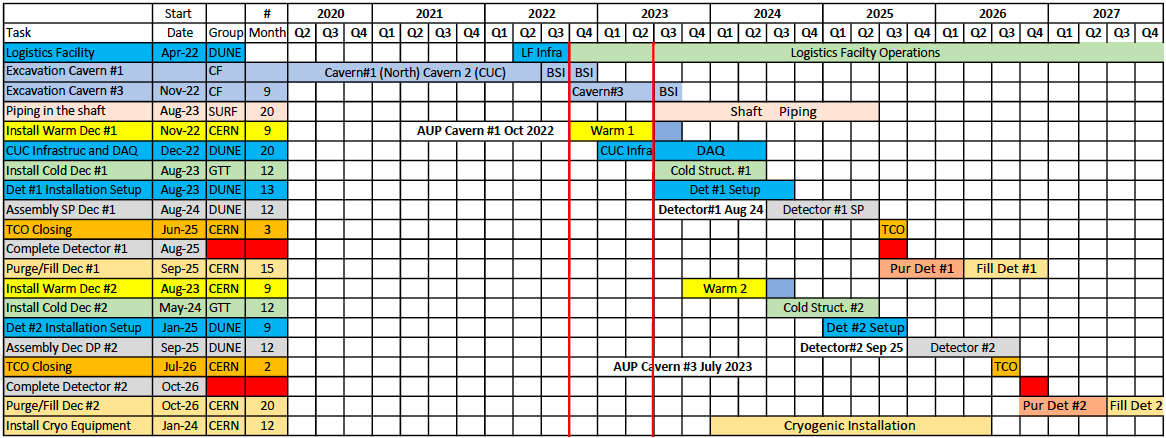
\includegraphics[width=0.85\textwidth]{summary-schedule-tc}
\end{dunefigure}

The ability of \dword{lbnf-dune} to meet this schedule depends 
critically on its ability to work within limitations on the total
number of people allowed in the underground areas at a given time.
In order to satisfy these limitations, careful balancing of the 
numbers of workers assigned to different concurrent tasks taking 
place within the different underground caverns is required.  
This is a particular challenge during the excavation period for 
the second detector cavern, which runs in parallel with cryostat
installation in the first detector cavern.  The \dword{jpo} works 
directly with its \dword{lbnf-dune} project parterns to manage 
and optimize the underground work schedule so that interferences 
between concurrent work efforts are minimized.

The underground cavern coordinator manages the contributions of 
the large technical team supporting the installation activities.
The size of the technical support team is anticipated to evolve  
over time to meet the needs of the specific installation tasks 
taking place.  The functions provided by the technical team 
supporting the work in the underground caverns includes the
following:

\begin{itemize}
  \item {material transport:} Unloading of materials from the 
        trucks arriving from the \dword{sdwf}, loading or rigging 
        of materials at top of Ross Shaft, unloading or rigging 
        of materials at bottom of Ross Shaft, and delivery of 
        materials from the bottom of shaft to the underground 
        caverns.        
  \item {cavern rigging operations:}  Storage of 
        components within the available spaces at the bottom 
        of the cavern and movement of materials as required to 
        execute the installation process (three rigging stages
        for detector installation are moving components into 
        clean room, integrating components within clean room, 
        and installing integrated elements inside cryostat).
  \item {installation technicians:}  General technician 
        support for specific installation activities. 
  \item {welders, survey crews, and cabling teams:}  Perform 
        specific tasks incorporated within each of the different 
        installation efforts.
  \item {electrical technicians, plumbers, and network 
        specialists:}  On-call support staff to modify systems 
        as work transitions from one stage to the next and to 
        address issues as they arise.             
\end{itemize}   
    
The organization responsible for managing contributions of 
the technical support team to the integration and installation 
activities taking place in the underground caverns is shown 
in Figure~\ref{fig:ctr_orgchart}.  The structure is illustrated
for the case of the largest anticipated workforce (approaching 
roughly sixty team members in total covering multiple shifts) 
for the periods with ongoing detector installation efforts.
These personnel support two 10-hour shifts on Mondays through 
Thursdays and a split day shift on the remaining days to cover 
any activities occuring over the weekends. 
\begin{dunefigure}[Common Technical Resources]{fig:ctr_orgchart}
  {Summary of the \dword{jpo}/\dword{sdsd} Common Technical Resources}
  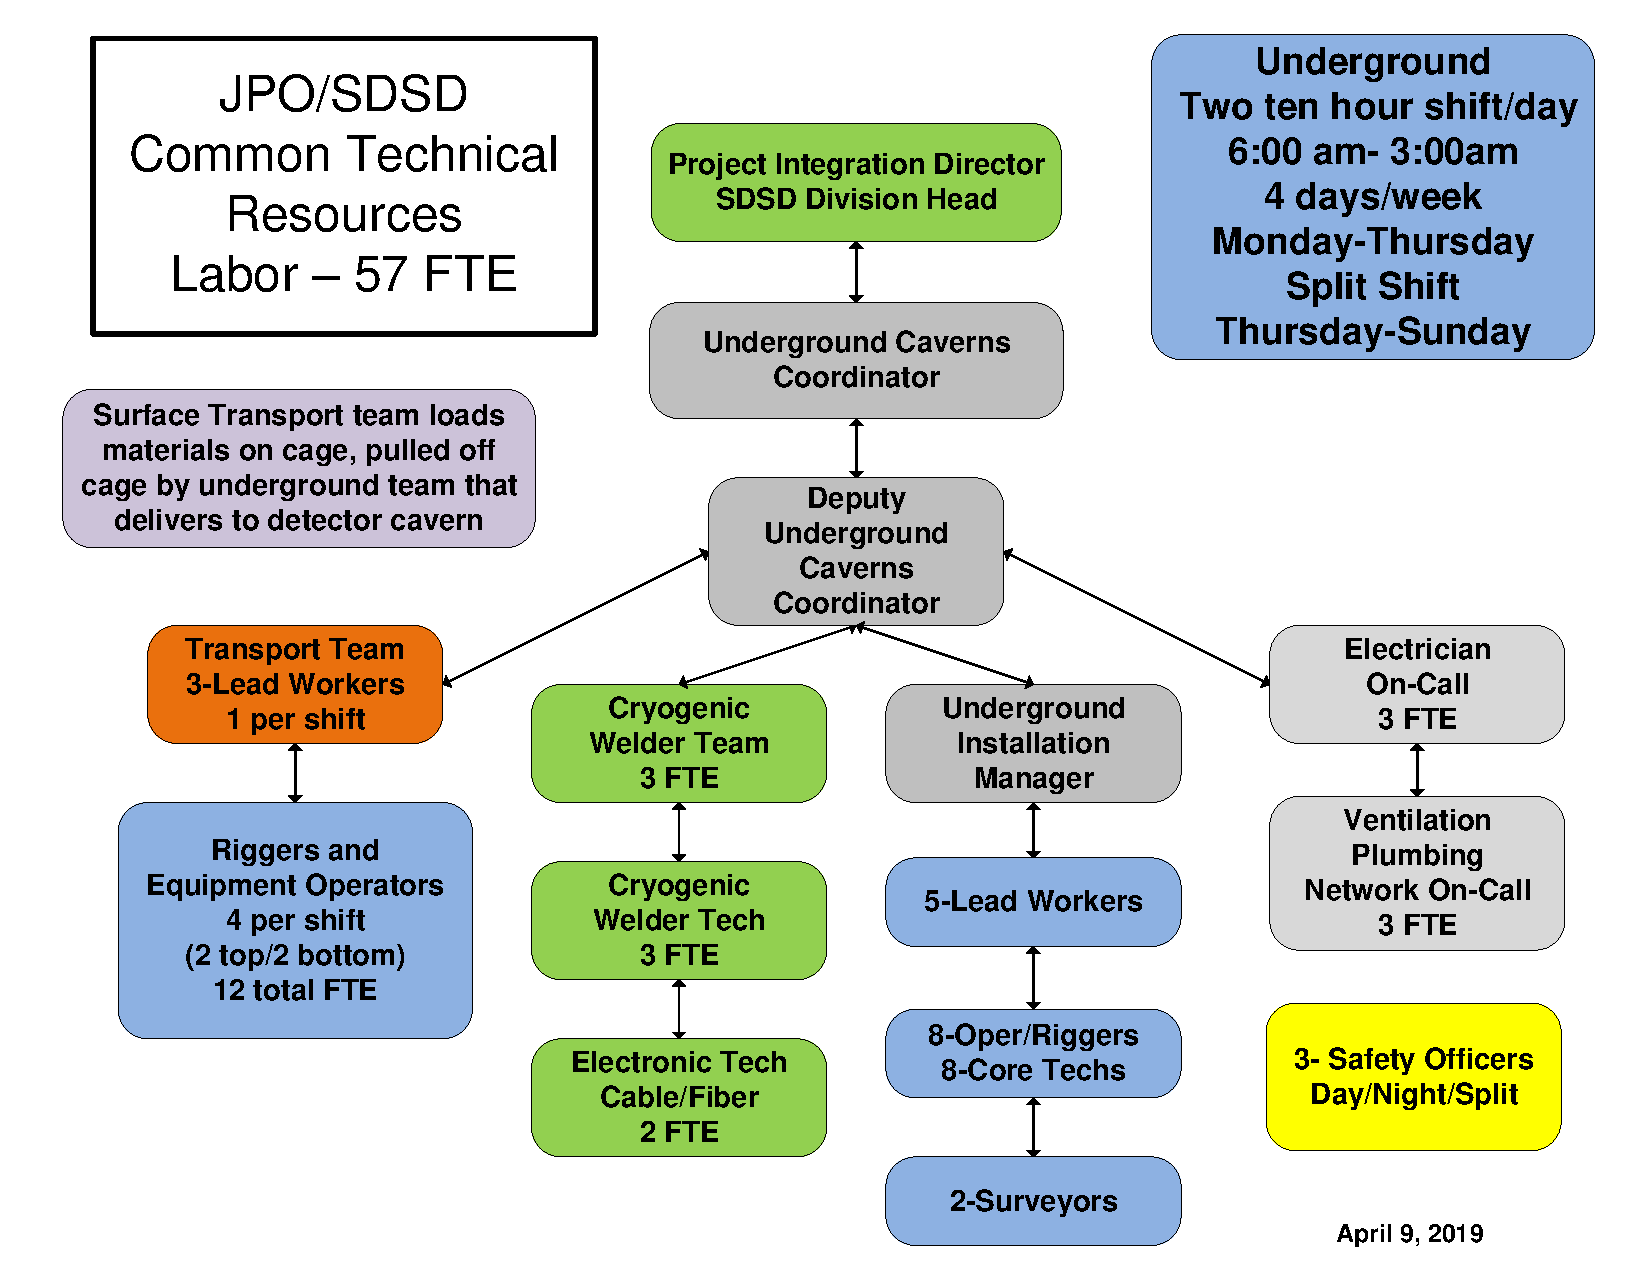
\includegraphics[width=0.95\textwidth]{Org_Technical_Resources-JPO-4-9-19.pdf}
\end{dunefigure}

On the surface at the start of each shift, there is a daily 
toolbox safety meeting and work assignment update. An hour 
separates the two shifts to allow ovelap between the shifts 
of the lead workers, safety officers, and other management 
team members, which facilitates the transfer of information 
from one shift to the next. The safety officer for each shift 
is responsible for conducting the safety discussion at the 
meeting and ensuring that all workers assigned to that shift 
have the proper trainings.

The team responsible for detector installation incorporates 
some members of the technical support team described above 
but also includes scientific and technical personnel from 
the \dword{dune} consortia.  The team is led by the detector 
installation manager who has three shift supervisors working 
with him or her to provide on-site coverage for every shift.
The management team works with the underground caverns 
coordinator to ensure that required technical support team 
members are available as needed and that required materials 
are delivered to the detector caverns on a schedule to keep
the installation effort moving forward.         

The management team supervises technical resources assigned to 
the detector installation effort and also works with the consortia 
team members to maximize the overall efficiency of the installation 
process.  The organizational structure used to manage the detector 
integration activities is shown in Figure~\ref{fig:uit_orgchart}.

\begin{dunefigure}[Underground Detector Integration/Installation Team]{fig:uit_orgchart}
  {The \dword{uit}}
  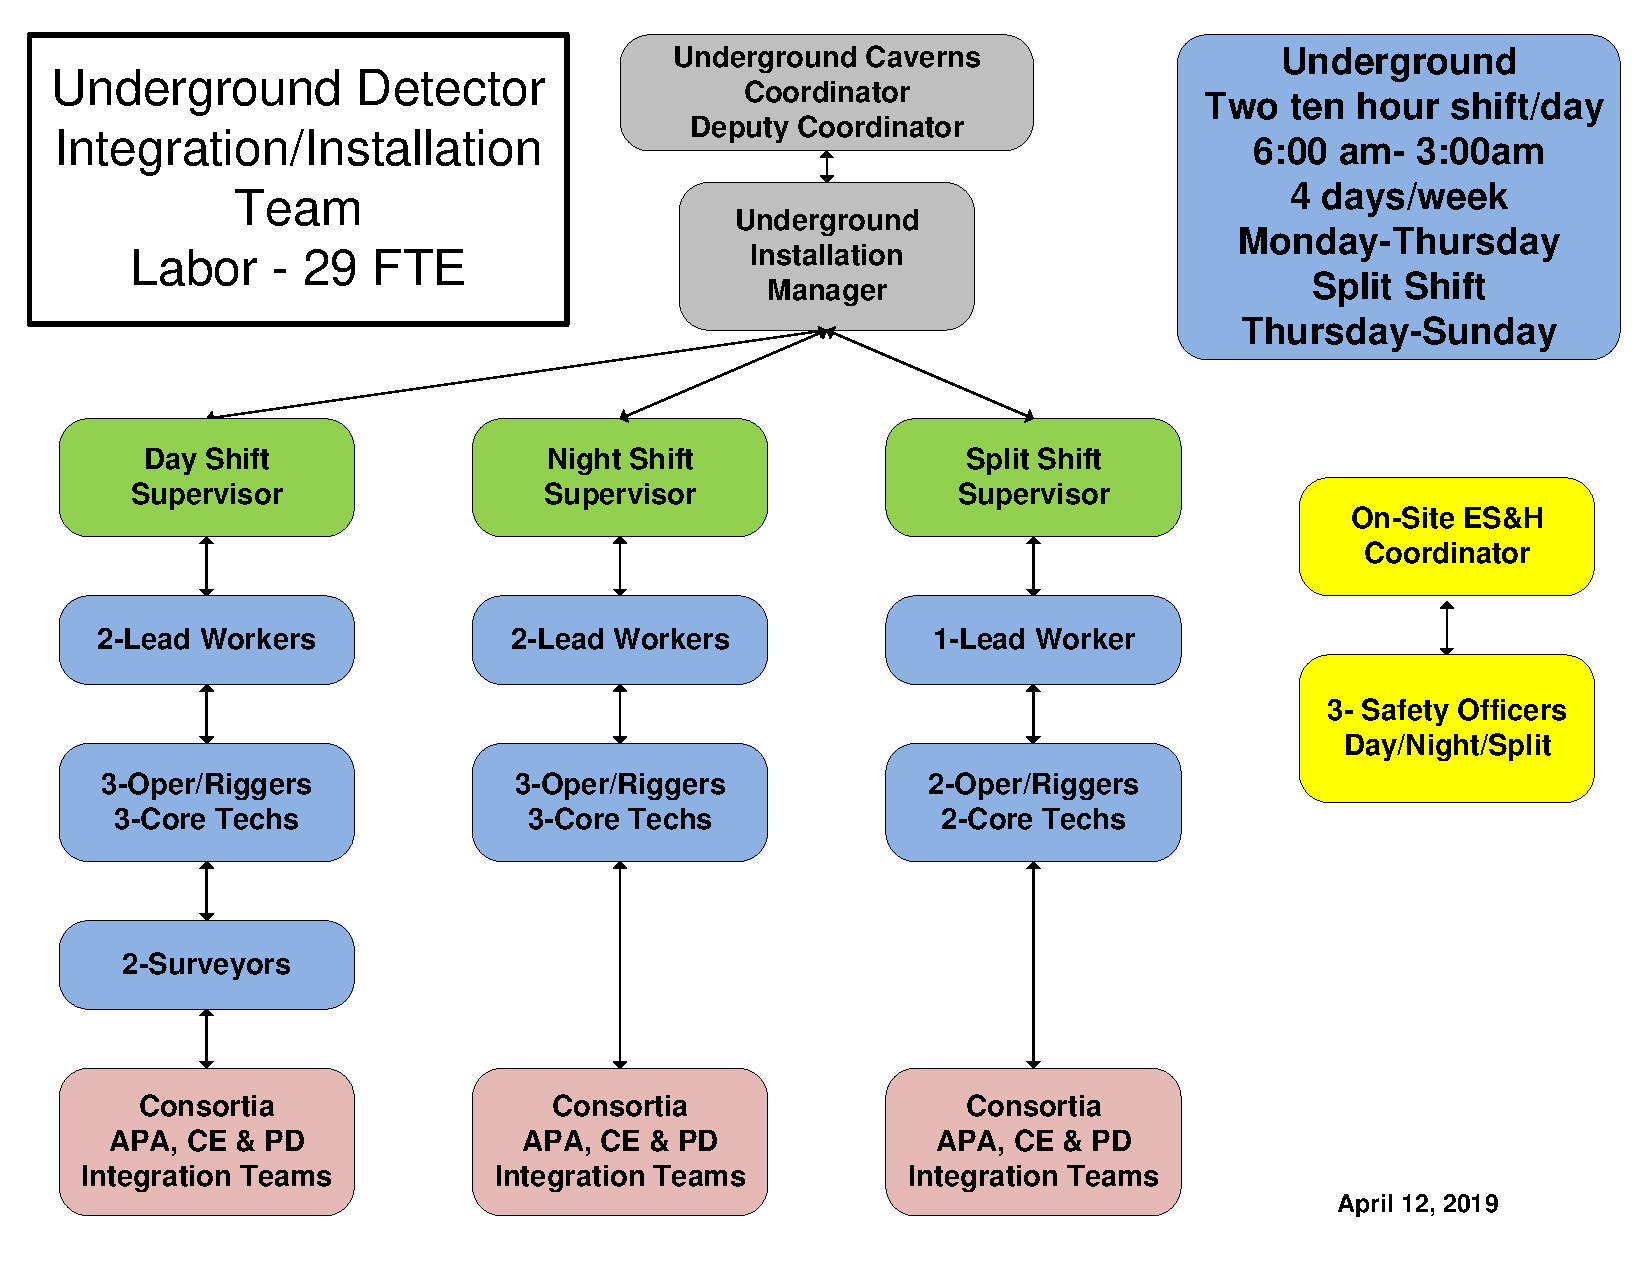
\includegraphics[width=0.95\textwidth]{Org_UIT-4-12-19.pdf}
\end{dunefigure}

The detector installation manager oversees all shifts but also 
covers as the supervisor for specific shifts as needed.  This 
individual serves as the direct contact with the underground caverns 
coordinator for obtaining required technical support
team members and organizing the delivery of needed materials 
into the detector caverns.  The detector installation manager 
attends all high-level meetings and is tasked with submitting
weekly progress reports.  This individual also works with the 
\dword{dune} consortia to manage the overall work schedule 
and ensure that the correct resources are in the right place
at the right time. 
    
The installation supervisors are working managers, trained as 
riggers and equipment operators to fill in as needed on their 
shifts.  They are fully trained in all installation procedures
and work with the consortia shift team members to keep the 
installation effort on schedule.  Installation Supervisors 
fill in for their lead workers as needed and are the primary 
points of contact for information that needs to be exchanged 
between shifts.  Lead workers are the main equipment operators 
and direct the technical support personnel assigned for their 
shift.  The lead workers are also trained in all installation 
procedures and provide assistance to the consortia work teams 
as needed.  

\subsection{Ash River}

\dword{ashriver} is the site of the \dword{nova} far detector in Ash River,
Minnesota, USA. The \dword{nova} far site detector hall offers a \SI{16.75}{m} 
deep pit with $\sim$\SI{300}{m$^2$} of floor space available for 
testing full-scale DUNE detector components.  The trial assembly 
work at Ash River focuses on mechanical tests to confirm designs,
including modifications originating from \dword{protodune}, 
and practice installation techniques.  As described below, the 
work is divided into three major phases.  The \dword{nova} Far 
Detector Laboratory is managed by the University of Minnesota 
and is partially funded through an operations grant from 
Fermilab.  Work performed at the Ash River site follows both 
university and Fermilab safety regulations, whichever is more 
stringent. University code officials approve all building permits, 
which include engineered drawings signed by an engineer registered 
in Minnesota. All hazard analyses and work procedure documents are 
approved by a joint safety committee with members drawn from both 
the University of Minnesota and Fermilab that includes specialists 
as needed.

The work at Ash River has four main goals:
\begin{itemize}
  \item verify that the \dword{dune} \dword{tpc} can be installed 
    in a safe and efficient manner,
  \item validate mechanical design changes made to the detector
    elements subsequent to \dword{protodune} operation,
  \item complete a set of procedural documents that will serve 
    as the basis for work to be performed underground at 
    \dword{surf}, and 
  \item serve as a training center for personnel who will 
    contribute to \dword{dune} integration and installation 
    efforts at \dword{surf}.
\end{itemize}

There is a full time staff of five personnel at Ash River including
a manager, deputy manager, and three experienced technicians.  The 
staff oversees operations of the \dword{nova} detector and performs 
the trial assembly studies of the \dword{dune} detector components.  
One of the three technicians also serves as the site safety officer 
and chairperson of the joint safety committee.  Two additional staff
members will be added in the near future to handle the additional 
workload associated with preparations for the \dword{protodune2} 
installation effort.  

\begin{dunefigure}[\threed model of the APA tower at Ash River]{fig:ashriver1}
  {\threed  model of the phase 1 trial assembly \dword{apa} tower at the \dword{nova} far detector lab in \dword{ashriver}.}
  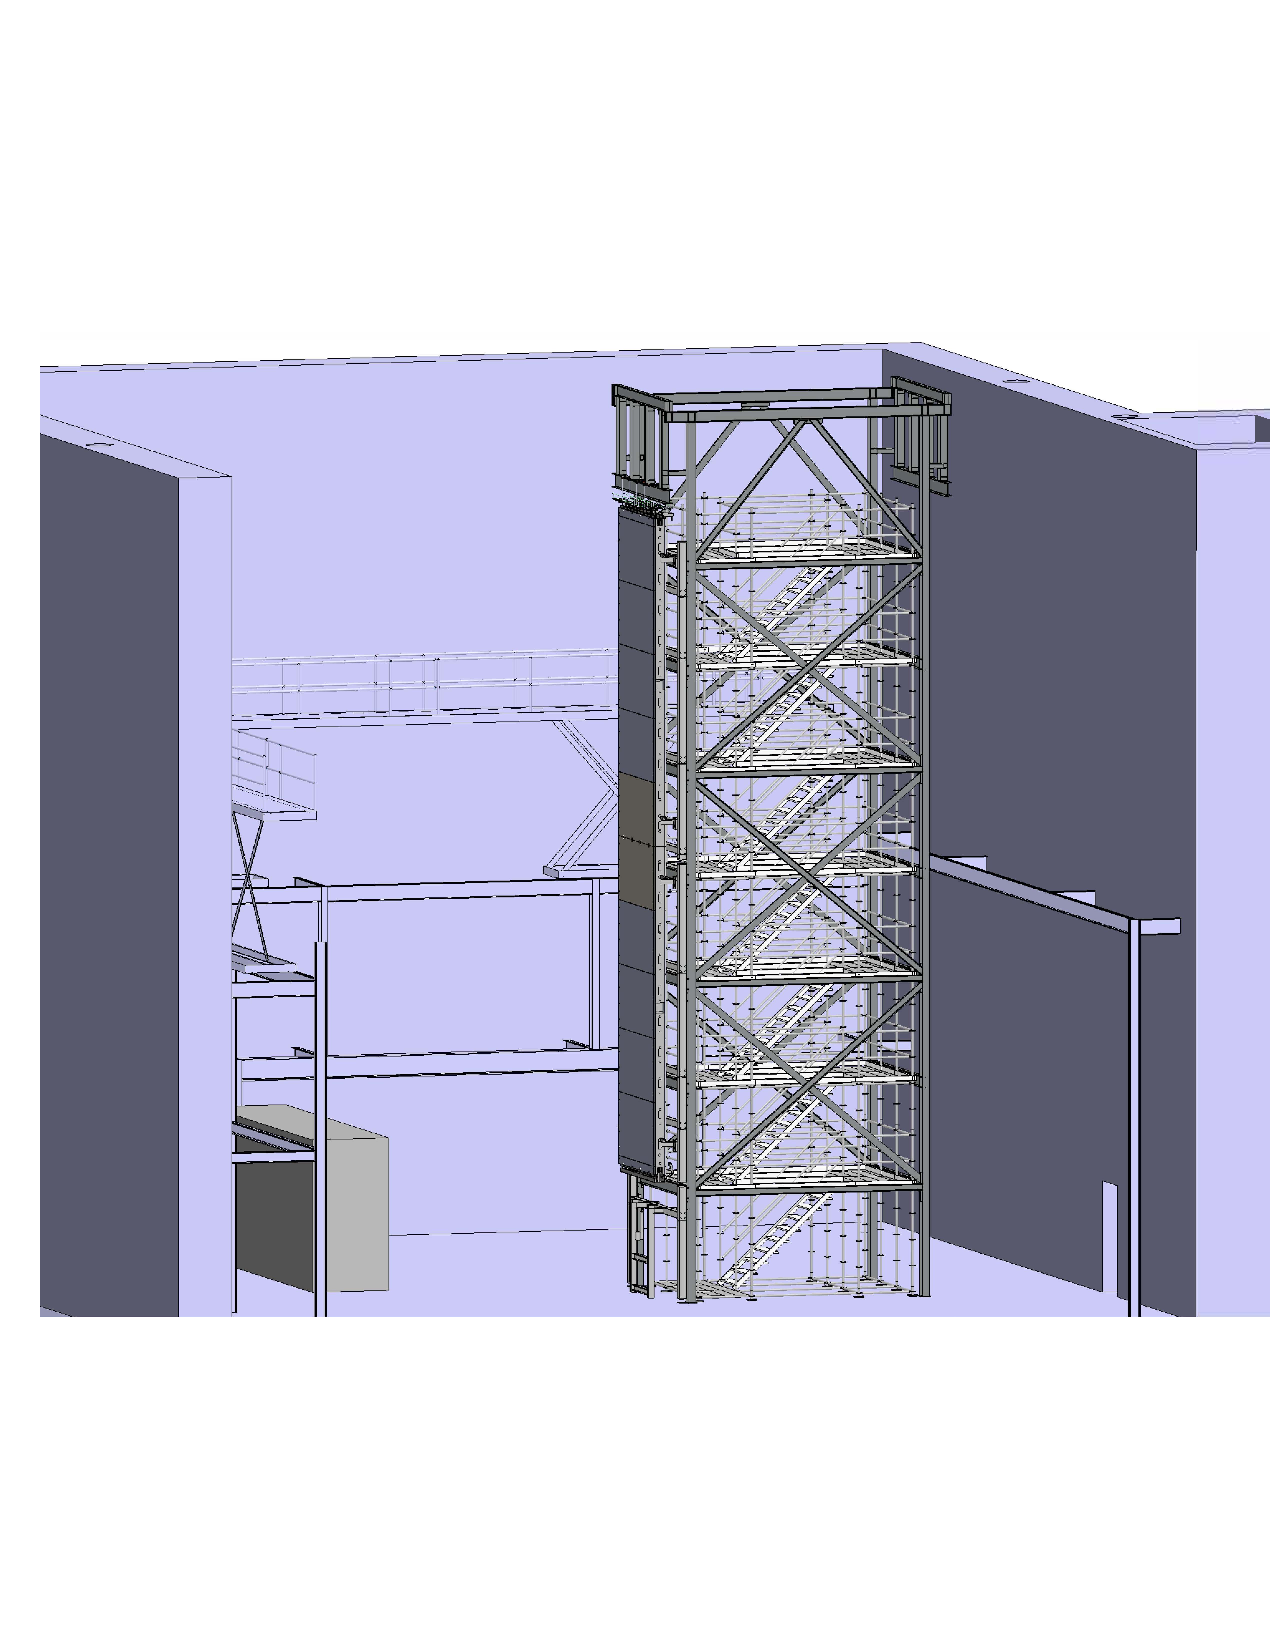
\includegraphics[width=0.65\textwidth]{APA_Tower_at_AshRiver.pdf}
\end{dunefigure}

The three major phases of \dword{ashriver} program are the following:

\begin{itemize}
  \item {Phase 0:} A vertical cabling test using two full-scale 
         \dword{apa} side tubes connected top to bottom and mounted 
         against a vertical column in the detector hall.  Using this 
         setup the proposed cable bundles have been run through the 
         tubes to see how well the designed conduit system functions.
         This work has led to several proposed modifications to the 
         designs which are currently being considered.  The older 
         \dword{protodune} trial assembly structure is concurrently 
         being used to perform mechanical tests of \dword{protodune2} 
         components. 
  \item {Phase 1:} A prototype of the \dword{dune} \dword{apa} 
         assembly tower using a steel frame large enough to hold a 
         commercial stair scaffold within its mid-section as shown 
         in Figure~\ref{fig:ashriver1} is being constructed.  The 
         tower is designed to test the process for connecting top 
         and bottom \dword{apa} pairs together and installing the 
         required cable bundles.  The next step will be to add a
         \dword{cpa} assembly station and test assembly procedures 
         for the updated \dword{cpa} designs.  A prototype 
         \dword{apa} shipping frame is also being constructed to 
         test the mechanical features of the shipping container 
         design.  
  \item {Phase 2:} A more complex steel structure will be 
         designed and fabricated to mock up the network of rails 
         and support strucutres used to install the \dword{dune}
         \dword{fd} modules including pieces of the \dword{dss}, 
         which sits inside the cryostat.  This structure as 
         illustrated in Figure~\ref{fig:ashriver2} will provide 
         a platform for performing more detailed tests of the 
         proposed detector installation plan.  Installation steps 
         to be tested include \dword{dss} installation, transfer 
         of \dword{tpc} components through the \dword{tco}, 
         installation of the \dword{tpc} end walls, cabling 
         through the cryostat penetrations, movement of the 
         \dword{apa} and  \dword{cpa} pairs into their final 
         positions, and deployment of the top and bottom field 
         cage modules.
\end{itemize}
\begin{dunefigure}[Phase 2 trial assembly at Ash River]{fig:ashriver2}
  {Phase 2 trial assembly at \dword{ashriver}.}
  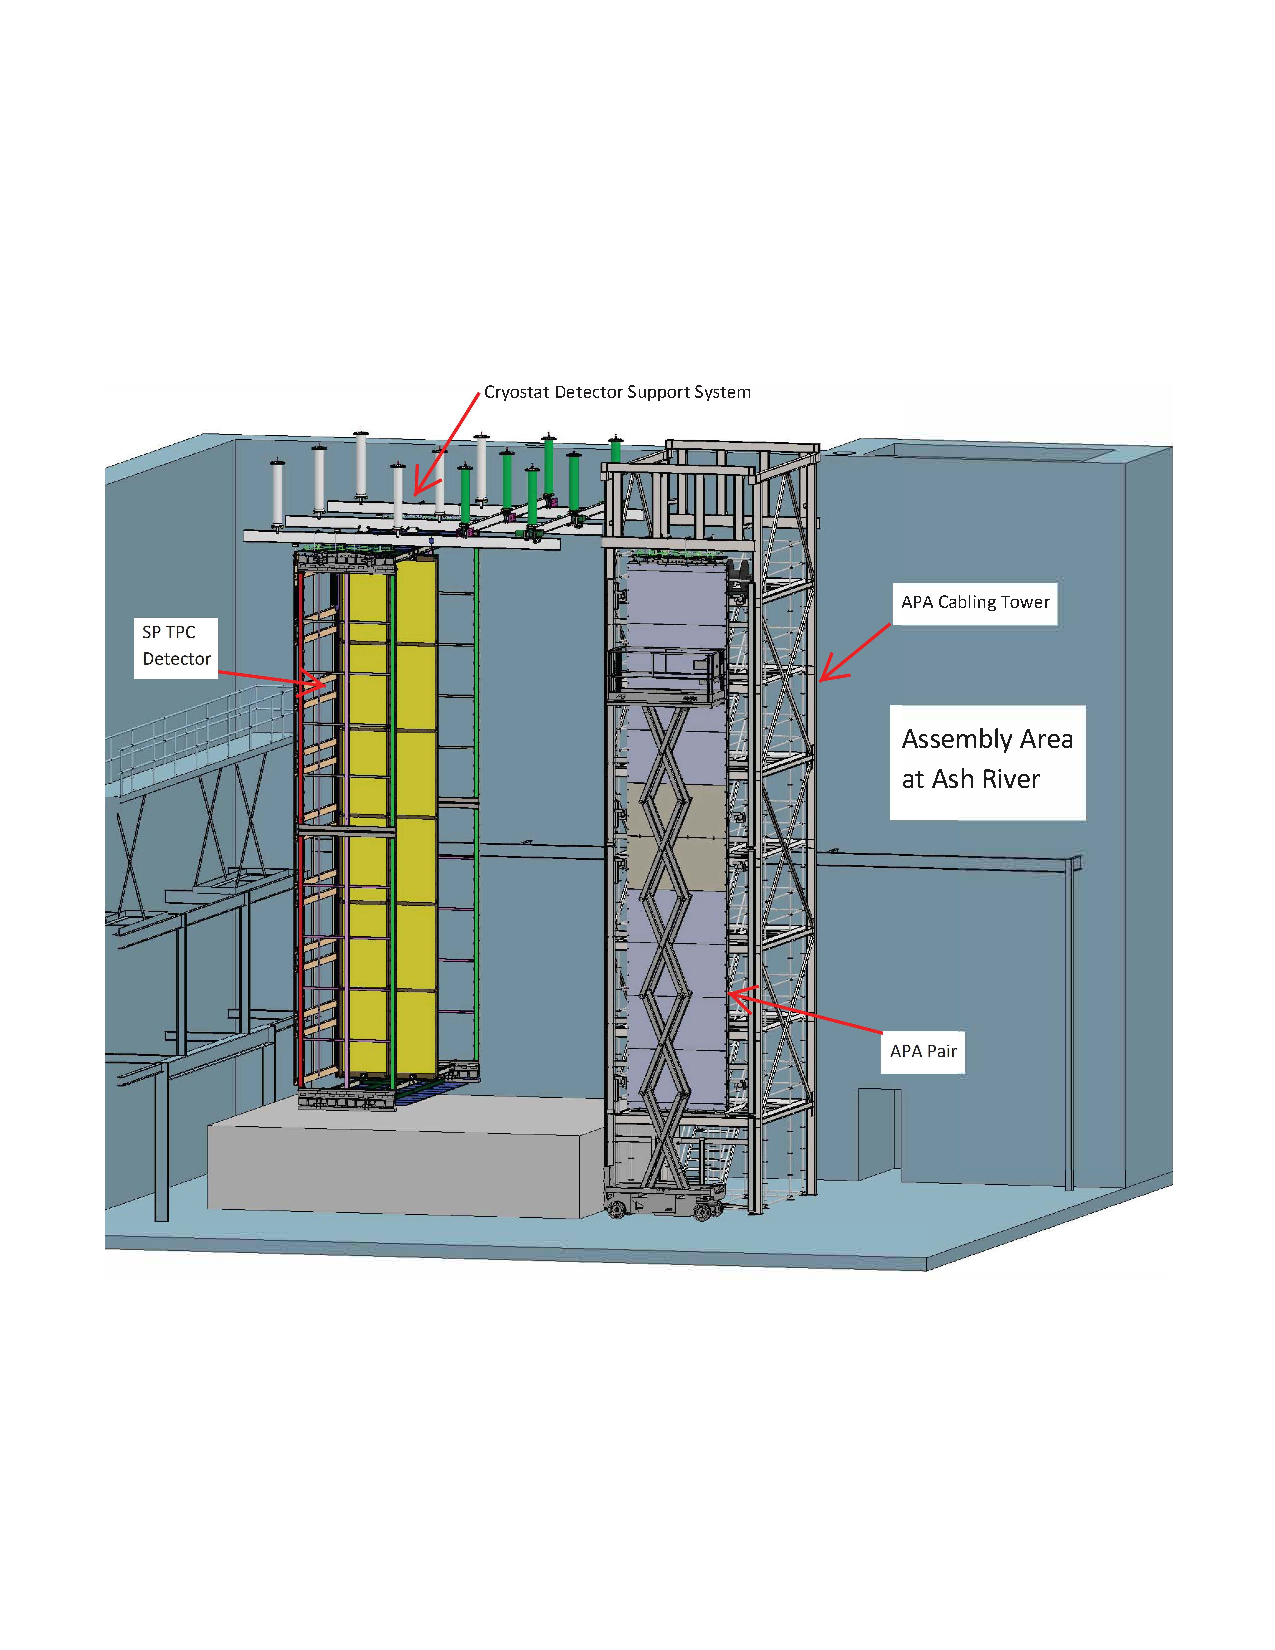
\includegraphics[width=0.65\textwidth]{Phase2_Trial_Assembly.pdf}
\end{dunefigure}

\section{South Dakota Services Division}
\label{sec:fdsp-coord-host_facility_services}

\dword{fnal} has established the \dword{sdsd} to support integration 
and installation activities in South Dakota. \dword{sdsd} will support 
these activities, which are the responsibility of the \dword{ipd}, 
by providing access to the required technical resources.  These 
resources include dedicated \dword{fnal} personnel sitting within 
the division and contracted labor provided through the division.   

\dword{sdsd} is responsible for badging and access to the leased 
areas at \dword{surf}. This includes providing and coordinating  
the trainings required to access surface and underground areas.  
\dword{sdsd} also takes on the responsibility for performing 
regular inspections and maintenance of \dword{lbnf-dune} equipment 
at \dword{surf} including lifts, conveyances, networking equipment, 
cooling and ventillation equipment, electrical power installations, 
life safety systems, and controlled access equipment.  Contracts 
that need to be written for conventional facilities procurements 
after the \dword{lbnf} conventional facilities contractor leaves 
the site will also be handled through the \dword{sdsd}.
